\label{sec:relam}

To reduce transition-driven uncertainty in aerothermodynamic heating
predictions, spatiotemporally homogenized direct numerical simulation
(DNS) was used to bound the turbulence-sustaining region on a blunt-bodied reentry
vehicle.  This chapter applies the ideas set forth in
\autoref{sec:detectingrelaminarization} to investigate which regions on the NASA
Orion MPCV thermal protection system cannot sustain turbulence during the peak
heating phase of return from the International Space Station.
%
That particular reentry scenario, described in \autoref{sec:orionmpcv},
was selected because of the availability of simulation data by
\citeauthor{Bauman2011Loose} and because of the upcoming NASA Exploration Flight
Test-1~\citep{SpaceCom20140317}.  Though that test will more closely resemble
the Orion MPCV returning from Earth's moon rather than the International Space
Station, it is nevertheless expected to produce experimental flight data against
which our simulation-based predictions might later be compared.
%
The method is described in \autoref{sec:relam_methods}.  Results and discussion
follow in Sections~\ref{sec:relam_results} and~\ref{sec:relam_discussion}.


%%%%%%%%%%%%%%%%%%%%%%%%%%%%%%%%%%%%%%%%%%%%%%%%%%%%%%%%%%%%%%%%%%%%%%%%%%%%%%
\section{Method}
\label{sec:relam_methods}

The method is broken into three sequential phases.
%
First, local conditions on the Orion MPCV heat shield surface during a fully
laminar reentry are quantified to identify the search space over which the
turbulence-sustaining study will proceed.
%
Second, spatiotemporal DNS are prepared at local conditions representative of
the heat shield edge with the goal of sustaining at least one statistically
stationary turbulent simulation.
%
Third, starting from a stationary simulation, the parameters are
adjusted to incrementally reflect conditions found increasingly closer to the
Orion MPCV stagnation point which are less likely to sustain turbulence.
%
If at this stage the flow relaminarizes, or at least enters a demonstrably
``quasi-laminar'' state~\citep{Sreenivasan1982Laminarescent}, the
turbulence-sustaining region boundary has been detected.
%
These three phases are elaborated in the remainder of this section.

%%%%%%%%%
% PHASE 1
%%%%%%%%%

In the first phase, an assumed laminar flow field over the Orion MPCV thermal
protection system was obtained from a simulation by P. T.
Bauman~\citep{Kirk2014Modeling,Bauman2011Loose}.  The laminar solution captured
the bow shock on the vehicle, accommodated the resulting high temperature
aerothermochemistry, included the curved MPCV geometry as the flow passed over
the thermal protection system, and incorporated a chemically reacting ablator
actively maintaining a cold wall despite the incoming enthalpy flux.  This
solution was post-processed to extract local boundary layer quantities of
interest along the thermal protection system symmetry plane, pictured in
\autoref{fig:cev_symplane}, producing the results already shown in
Figures~\ref{fig:cevisslam_summary1} and~\ref{fig:cevisslam_summary_fpg}.
%
Those quantities are the Reynolds number based on momentum thickness
$\Reynolds[\theta]{}$, the edge Mach number $\Mach[e]{}$, the favorable pressure
gradient strength as measured by the parameter
$p_{e,\xi}^{\ast}$~\eqref{eq:defnpexi}, the wall blowing velocity normalized by
the friction velocity $v_w^{+} = v_w / u_\tau$, the coldness of the wall
relative to the boundary layer edge $T_e/T_w$, the Prandtl number $\Prandtl$,
and the ratio of specific heats $\gamma = C_p / C_v$.
%
Out of the many possible pressure gradient parameters
that the study could target,
$p_{e,\xi}^{\ast}$ was chosen motivated by the needs of the inviscid base flow
design process of Appendix~\ref{sec:radialflow} in conjunction with that
procedures' successful application in \autoref{sec:bldata}.

At each location on the thermal protection system surface the above quantities
collectively characterize the subset of the peak heating boundary layer physics
that can be captured by the governing equations from \autoref{sec:goveqn}.
%
Mapping Bauman's complex, multiphysics solution onto this comparatively simple
Navier--Stokes formulation crudely approximates high temperature reacting air by
a perfect gas.  Further, variations in the Prandtl number and ratio of specific
heats are neglected and replaced by constant air values $\Prandtl=0.7$ and
$\gamma=1.4$.  A power law viscosity was assumed with exponent
$\beta=\nicefrac{2}{3}$ based on fitting high temperature air data as shown in
\autoref{fig:Svehla1962}.
%
At the end of the phase, the entire reentry scenario had been reduced to a
single mapping of the distance leeward from the vehicle's stagnation point
to the five nondimensional local conditions:
$\Reynolds[\theta]{}$, $\Mach[e]{}$, $T_e/T_w$, $v_w^{+}$, and
$p_{e,\xi}^{\ast}$.

\begin{table}[p]
\makecommand{\z}{\phantom{0}}  % Facilitates column alignment
\makecommand{\Z}{\phantom{.0}} % Ditto
\centering
\caption[%
    Selected locations from the fully laminar Orion MPCV TPS simulation
]{%
    Selected reacting boundary layer conditions from the symmetry plane
    on a fully laminar Orion MPCV thermal protection system simulation
    depicted more fully in Figures~\ref{fig:cevisslam_summary1}
    and~\ref{fig:cevisslam_summary_fpg}.  Column ``Location'' indicates
    the number of meters leeward of the stagnation point where the
    conditions are found.\label{tbl:cevisslam_detail1}
}
\begin{tabular}{cccccc}
Location                              &
$\textrm{Re}_{\theta}$                & % Re_theta
$\textrm{Ma}_{e}$                     & % Ma_edge
$T_{e}/T_w$                           & % T_ratio
$v_w^{+}$                             & % v_wallplus
\raisebox{0.10ex}{$p_{e,\xi}^{\ast}$}   % p_exi
\\
\toprule\toprule
%Location  &  Re_theta  &  Ma_edge  &  T_ratio &  v_wallplus  &  p_exi           \\
4.134~m    &  223       &  1.152\z  &  4.285   &  0.007178    &  \num{-0.01235}  \\
3.199~m    &  225       &  0.8986   &  4.262   &  0.008387    &  \num{-0.01019}  \\
2.299~m    &  177       &  0.6597   &  4.182   &  0.009765    &  \num{-0.01269}  \\
1.389~m    &  114       &  0.4112   &  4.129   &  0.01225\z   &  \num{-0.01793}
\end{tabular}
\end{table}

%%%%%%%%%%%%%%%%%%%%%%%%%%%%%%%%%%%%%%%%%%%%%%%%%%%%%%%%%%%%%%%%%%%%%%%%%%%%%%
%%%%%%%%%%%%%%%%%%%%%%%%%%%%%%%%%%%%%%%%%%%%%%%%%%%%%%%%%%%%%%%%%%%%%%%%%%%%%%

\begin{table}
\makecommand{\z}{\phantom{0}}  % Facilitates column alignment
\makecommand{\Z}{\phantom{.0}} % Ditto
\centering
\caption[%
    Input parameters used in the relaminarization study to obtain Orion
    MPCV-like boundary layer conditions
]{%
    Suzerain v0.1.6.34-r45407 input parameters found to approximately
    match local boundary layer conditions at locations in
    \autoref{tbl:cevisslam_detail1}.
    %
    For all cases, $\textrm{Pr} = \mu C_p / \kappa = 0.7$, $\alpha=0$ in
    $\mu_B=\alpha\mu$, $\beta=\nicefrac{2}{3}$ in $\mu / \mu_0={\left(T /
    T_0\right)}^\beta$, and $\gamma = C_p / C_v = 1.4$.
    %
    Extents were $L_x/l_0=10$, $L_y/l_0=2.5$, $L_z/l_0=3$ employing a
    piecewise-quintic B-spline basis with $N_y=192$ collocation points.
    %
    Column ``Advance'' reports which linear implicit operator and
    time step safety factor governed time advance.
    %
    Refer to Tables~\ref{tbl:table_turb_hbl}
    through~\ref{tbl:table_turb_hbl_fpg} for other column
    definitions.\label{tbl:cevisslam_inputs}
}
{\renewcommand{\tabcolsep}{0.345em}
\begin{tabular}{cccccccccc}
Location                                        &%  Location
$\textrm{Re}$                                   &%  Re
$\textrm{Ma}$                                   &%  Ma
$\tanh$                                         &%  tanh
$\operatorname{gr}_{t_0}\!\left(\Delta\right)$  &%  grdelta
$T_w/T_0$                                       &%  Tw
$v_w/u_0$                                       &%  vw
\raisebox{0.10ex}{$p_{e,\xi}^{\ast}$}           &%  p_ex
\multicolumn{2}{c}{Advance}                      %  implicit,safetyfactor
\\
\toprule\toprule
% DATA DRAWN FROM CASES relam${CASE}/last/restart00000.h5
%Location &  Re     &  Ma       &  tanh  &  grdelta    &  Tw      &  vw             &  p_ex            &  implicit  &  safetyfactor  \\
4.134~m   &  1535   &  1.152\z  &  2.2   &  0.02175    &  0.2333  &  \num{1.99e-4}  &  \num{-0.01234}  &  Y         &  0.35\z        \\
3.199~m   &  1475   &  0.8985   &  2.2   &  0.016\z\z  &  0.2346  &  \num{2.20e-4}  &  \num{-0.01019}  &  XYZ       &  0.2\z\z       \\
2.299~m   &  1100   &  0.6598   &  2.0   &  0.01\z\z\z &  0.2391  &  \num{2.68e-4}  &  \num{-0.01269}  &  XYZ       &  0.2\z\z       \\
1.389~m   &  \z800  &  0.4113   &  2.0   &  0.0035\z   &  0.2422  &  \num{3.68e-4}  &  \num{-0.01793}  &  XYZ       &  0.175
\end{tabular}}
\end{table}


%%%%%%%%%
% PHASE 2
%%%%%%%%%

In the second phase, the direct numerical simulation code Suzerain was used to
prepare spatiotemporally homogenized flow fields at several ``locations'' from
the reentry-specific mapping described above.  Only one
location at the heat shield edge was required to proceed to the third phase.
%
However, as multiple independent locations easily could be made ready
simultaneously, four locations roughly quadrisecting the search space were
prepared.

\autoref{tbl:cevisslam_detail1} documents the four selected locations.
%
Locations 3.199~m and 4.134~m correspond to $\Reynolds[\theta]{}=223$ and
$225$ variants of the scenario conditions found in \autoref{sec:bldata}
simulations t3.199 and t4.134, respectively.
%
Both of these locations were expected to sustain turbulence based on the
\citet[\textsection{}3.2]{Spalart1988Direct} finding that his constant
viscosity, homogenized sink flow simulations quickly relaminarized below
$\Reynolds[\theta]{}=330$ because 3.199~m and 4.134~m have appreciably higher
momentum Reynolds numbers when evaluated using wall viscosity
(\autoref{fig:cevisslam_summary1}).
%
Having cases at subsonic and supersonic conditions was done to hedge against the
possibility of either the spatiotemporal homogenization or the inviscid base
flow design procedure becoming numerically problematic if the third phase of
this study dictated iteratively adjusting a simulation across
$\Mach[e]{}=1$.\footnote{%
    Concern about the spatiotemporal homogenization in supersonic circumstances
    arose based on observations reported at the end of
    \autoref{sec:bldata_stats}.  Concerns about the base flow procedure stemmed
    from the design procedure of Appendix~\ref{sec:radialflow_match} driving the
    nozzle radius $R$ to large values as $\Mach[e]$ approaches one from either
    direction.
}
%
Either location 2.299~m or 1.389~m was hypothesized to relaminarize.

At each of those four locations the MPCV-derived data in
\autoref{tbl:cevisslam_detail1} furnished fixed values for only
the Suzerain code input parameters $\Mach\approx{} u_{99} /
a_{99}$, $T_w/T_0$, and $p_{e,\xi}^{\ast}$.
%
As doing so had proved successful for \autoref{sec:bldata},
boundary layer thickness $\delta_{99}/l_0=1$ was chosen as a
target to be achieved indirectly by adjusting the slow growth rate
$\operatorname{gr}_{t_0}\!\left(\Delta\right)$.
%
When that condition is met, the nondimensional formulation in conjunction with
the inviscid base flow design procedure \emph{a priori} causes $\rho_{99} /
\rho_0$, $u_{99} / u_0$, and $T_{99} / T_0$ to all be nearly one.
%
Appropriate values for the remaining code inputs $\Reynolds\approx \rho_{99}
u_{99} \delta_{99} / \mu_{99}$, $\operatorname{gr}_{t_0}\!\left(\Delta\right)$,
and $v_w/v_0$ had to be discovered.
%
An elegant way to discover suitable settings would be to invert for the
appropriate values using a spatiotemporally equipped turbulence model
implementation properly calibrated for the current context.
%
A less elegant way would be to iteratively seek values with such a tool in lieu
of the more complicated inversion procedure.
%
The inelegant way used in this study was to perform exploratory simulations to
manually acquire the needed values by iteratively adjusting code input
parameters until the desired stationary behavior was obtained.
%
\autoref{tbl:cevisslam_inputs} reports those parameters.
%
To conserve compute resources, these computations used coarse streamwise and
spanwise resolution (for example, $\Delta{}x^{+}\approx{}30$) but production
wall-normal bases with $y^{+}_1$ and $y^{+}_{10}$ comparable or better than
those in \autoref{tbl:table_turb_hbl}.
%
Final tests to ensure the parameters appearing in \autoref{tbl:cevisslam_inputs}
were robust on near-production grids (for example, $\Delta{}x^{+}\leq{}25$ and
$\Delta{}z^{+}\leq{}15$) yielded unexpected results which will be conveyed in
\autoref{sec:relam_results_refine}.

%%%%%%%%%
% PHASE 3
%%%%%%%%%


For the third phase, the code input parameters shown in
\autoref{tbl:cevisslam_inputs} were used to adjust a fully turbulent field so
it matched the target conditions derived from MPCV data.
%
A known-good turbulence field was required to ensure that the relaminarization
study was seeded with a reasonable approximation of boundary layer physics.
Moreover, turbulent conditions are a ``large perturbation'' with respect
to a relaminarized flow per the energy method ideas discussed in
\autoref{sec:energyperturbationtheory}.
%
That adjustment process
is simpler if the initial field already resembles the target flow conditions.
Simulations t3.199 and t4.134 from \autoref{sec:bldata} were designed to serve
exactly that purpose.  They differed from \autoref{tbl:cevisslam_detail1} locations 3.199~m and 4.134~m only in
their $\Reynolds[\theta]{}$ magnitudes.
%
Results starting from these initial conditions will appear in
\autoref{sec:relam_results_turb}.

Though the collapse of turbulent fluctuations and relaminarization can be a
quick process in spatially evolving boundary layers subjected to pressure
gradients~\citep{Mukund2006Relaminarization} and spatially homogenized boundary
layers~\citep[\textsection{}3.2]{Spalart1988Direct}, it was uncertain if that
would also be true for the \citet{Topalian2014Spatiotemporal} spatiotemporal
homogenization or if this slow growth formulation would bring about an
extended ``quasi-laminar'' state~\citep{Narasimha1979Relaminarization,
Sreenivasan1982Laminarescent} that would prove difficult to identify.  An
extended relaminarization process would retard our ability to incrementally move
to locations nearer the stagnation point because it would force us to simulate
each station for a longer duration to ensure we did not accidentally pass over
the critical location.
%
For this reason, an \emph{in situ} capability to assess the strength of the
turbulence by monitoring the temporal trace of relevant quantities was added to
Suzerain.  Following findings by \citet{Cal2008Similarity}, the code was
augmented to frequently output maxima values and locations for absolute values
of Reynolds-averaged and Favre-averaged stress tensor components.  Output of the
wall-normal location and value of the peak streamwise- and spanwise-averaged
production term as well as its integrated magnitude was also added.  These
monitors permitted early identification of relaminarization precursors.

An insufficiently large computational domain and inadequate spatial resolution
tend to cause turbulent fluctuations to persist.  The former introduces
artificially long correlation lengths and the latter does not permit turbulent
kinetic energy to be dissipated properly.  Either effect would likely cause the
study to incorrectly detect the turbulence-sustaining region.  Plans were laid
to repeat the final stages of the detection process with a larger domain and
improved resolution.

%An early draft:
%\begin{enumerate}
%\item Given scenario parameters/base flows, compute stationary 1D laminar
%profiles at each location on the CEV.  These local heat flux at the wall
%magnitudes serve as canaries for when relaminarization is occurring.
%Initially, we say the flow has relaminarized if a turbulent case's heat flux at
%the wall is within 10\% of these local laminar results.
%\item Choose a location A possessing the maximal $\Reynolds[\delta^\ast]$ among
%all locations.  Initialize a small box simulation at reasonable resolution (per
%Victor/Wu) for A's base flow.  Run until stationary.  If not stationary, freak
%out.
%\item Choose a location B a small distance from the stagnation point where
%turbulence is not expected.  Take stationary field from A and instantaneously
%adjust scenario parameters to match location B.  Run B until it relaminarizes
%noting the amount of simulation time necessary to achieve that decay as
%measured relative to wall heat flux to laminar wall heat flux ratio.  If B does
%not relaminarize or takes too long, freak out.
%\item Partition A to B into O(10) segments [A0, A1), [A1, A2), ..., [A8, A9)
%where A0 = A, A9 = B.
%\item Set i = 0.
%\item Take stationary field from A(i-1) and instantaneously adjust to match
%conditions at A(i).  Run simulation.
%\begin{enumerate}
%    \item If A9 = B reached and flow hasn't relaminarized, freak out.
%    \item If run becomes stationary, i+=1 and repeat 6.
%    \item If run relaminarizes, [A(i-1), A(i)) likely contains the
%    relaminarizing cusp.  Continue.
%\end{enumerate}
%\item Partition A(i-1) to A(i) into O(10) segments and repeat steps 6 and 7 on
%this finer gradation.
%\item Presumably now, for the chosen box and grid, we know exactly where the
%behavioral cusp is.
%\item Initialize a new small box run at A on a finer resolution.  Quickly move
%to confirm behavioral cusp with finer resolution.
%\item Initialize a new big box run at modest resolution.  Quickly move to
%confirm behavioral cusp with larger box size.
%\item If no cause for freaking out, declare success.
%\end{enumerate}
%
%What actually happened:
%\begin{enumerate}
%\item Took turbulent fields from prior chapter, coarsened, and aimed for
%    conditions 1.389, 2.299, 3.199, and 4.134 meters leeward of the stagnation
%    point.
%\begin{enumerate}
%    \item Location 1.389 promptly relaminarized
%    \item Location 2.299 relaminarized
%    \item Location 3.199 relaminarized with a small dwell
%    \item Location 4.134 relaminarized over a timeframe of nearly 9 turnovers
%    \item STARTHERE
%\end{enumerate}
%
%\end{enumerate}

%%%%%%%%%%%%%%%%%%%%%%%%%%%%%%%%%%%%%%%%%%%%%%%%%%%%%%%%%%%%%%%%%%%%%%%%%%%%%%
\section{Results}
\label{sec:relam_results}

Two distinct sets of results are presented.
%
The first set of results, found in \autoref{sec:relam_results_refine}, conveys
the unexpected behavior observed when coarse, fluctuation-sustaining exploratory
simulations were refined to production resolutions.
%
The second set of results, appearing in \autoref{sec:relam_results_turb},
investigates relaminarization using fully turbulent fields from
\autoref{sec:bldata} so that the initial conditions represent boundary layers
like those found on the Orion MPCV.


%%%%%%%%%%%%%%%%%%%%%%%%%%%%%%%%%%%%%%%%%%%%%%%%%%%%%%%%%%%%%%%%%%%%%%%%%%%%%%
\subsection{Results from Refining Coarse Exploratory Simulations}
\label{sec:relam_results_refine}

All four coarse simulations performed to discover inputs for
\autoref{tbl:cevisslam_inputs} relaminarized when refined to
$\Delta{}x^{+}\leq{}25$ and $\Delta{}z^{+}\leq{}15$.  The relaminarization
events were not cleanly captured--- initially they were thought to be merely
undesirable drift relative to target conditions which prompted us to adjust code
inputs partway through each event.  After appreciating what had occurred, the
process was repeated but, unlike before, without any adjustments to code inputs
once the simulations were underway.

Figure~\vref{fig:relam4134} shows the temporal evolution of the supersonic coarse
location 4.134~m simulation immediately after refinement.  The earliest time
shown is when the field was refined to $\Delta{}x^{+}\approx{}18.7$ and
$\Delta{}z^{+}\approx{}11.2$ ($N_x = 256$ and $N_z=128$) while holding the
wall-normal basis constant.  As the projection onto a larger Fourier basis is an
exact operation, the refinement does not perturb the flow but it does permit the
solution to populate higher wavenumbers and thereby gain additional dissipative
capability.  The upper six subplots in \autoref{fig:relam4134} show the desired
location-specific conditions as a horizontal dashed line and the actual
simulation evolution in blue curves.
%
The mean flow in the freestream approximately traverses the streamwise extent of
the domain once every 10 time units because because $u_{99}/u_0\approx{}1$ and
$L_x/l_0=10$.
%
For example, $\Reynolds[\theta]$ starts
out slightly too high, grows slowly until just before nondimensional time index 120,
and then gradually drops.  Proceeding down the subplots, the edge Mach number
is seen to be very close to target while the temperature ratio is low.  Wall
blowing $v_w^{+}$, the pressure gradient parameter $p_{e,\xi}^\ast$, and the
boundary layer thickness all match the desired values.

The lower three
subplots in \autoref{fig:relam4134} show turbulence diagnostics.
%
The uppermost of the three is the instantaneous mean turbulent production $-
\bar{\rho} \widetilde{u''\otimes{}u''} : \nabla\tilde{u}$ averaged across all
spatial directions.  It is nondimensionalized by edge state similarly to
$\Reynolds$ and $\Mach$ defined earlier.  Production begins to drop
around time 100.  The next subplot down is the pointwise maximum absolute values
of each component of the Favre-averaged stress tensor.
%
To permit visualizing both early- and late-time behavior, the logarithm of the
absolute values are plotted.   The data is clipped below $10^{-8}$ which only
obscures low magnitude information at late times ($t>240$).
%
After $t>120$ the fluctuation magnitudes slowly drop because of the
extra dissipation available due to the increased spatial
resolution.  As \citet{Cal2008Similarity} reported, the $vv$ and $uv$ curves
decay sharply after the integrated production tails off at $t=180$.  The final
curve is the skin friction factor which decays to a nearly constant value by
$t>300$.
%
Basing $\delta_{99}$ and $u_\tau$ determinations on the initial boundary layer
character, it took roughly 4.2 eddy turnovers\footnote{Computed from $(t_f - t_i) u_\tau / \delta_{99}$.}
from the start of the study until relaminarization precursors appear
and another 1.8 turnovers to reach $t=180$ where the flow
clearly is relaminarizing.

\autoref{fig:relam3199} shows the temporal evolution of the
coarse location 3.199~m simulation immediately after refinement to
$\Delta{}x^{+}\approx{}18.0$ and $\Delta{}z^{+}\approx{}10.8$ ($N_x = 256$
and $N_z=128$).  The $\Reynolds[\theta]$ dips below target, the
$T_e/T_w$ is again low, but the other indirectly controlled parameters
in the upper six subplots
oscillate about the desired values.  Turning to the lower turbulence diagnostics, the
integrated production is quite variable and shows intermittent periods
of decreased production.  The maximum density-weighted stress tensor
components show several relaminarization precursor signatures with the
most pronounced at $t=400$, $t=800$, and $t=1100$.  These are also
seen in the integrated production and skin friction traces.  At each of
those times, however, the fluctuations again kick up and the flow briefly
appears turbulent from these plots.  The dwell time between them is
10.2 and 8.7 eddy turnovers which is longer than the O(6.5) turnover
statistical ensembles gathered in \autoref{sec:bldata}.
%
These three diagnostic subplots show evidence of a characteristic frequency
which may be related to the time scale of the structural interactions
responsible for reinvigorating the fluctuations after each window of decay.
%
From initialization until relaminarization,
36.3 eddy turnovers passed.

\autoref{fig:relam2299} shows the evolution of the coarse location 2.299~m
simulation after refinement to $\Delta{}x^{+}\approx{}14.1$ and
$\Delta{}z^{+}\approx{}8.5$ ($N_x = 256$ and $N_z=128$).  The flow does not
relaminarize over the 23.2 turnovers shown though short lulls appear in the
production during which the stress tensor component magnitudes smooth out due
to dissipation and the skin friction decreases.  Glancing at the top portion of
the figure, however, reveals that wall blowing is too weak and the favorable
pressure gradient too strong on account of the growth rate parameter not
achieving $\delta_{99}\approx{}1$.

\autoref{fig:redux2299} rectifies the target condition mismatch by proceeding
with the new input parameters documented in the figure caption.
Those new parameters took three attempts to discover.
The $T_e/T_w$
target is still too low and the wall blowing just slightly too high, but
overall the disagreement with all target conditions, in particular
the pressure gradient, was remedied.  The production, stress tensor components,
and skin friction continue to show intermittency but location 2.299~m sustained
turbulence for another 23.4 turnovers.  It was unclear whether or not
the intermittency would continue indefinitely or if, eventually,
2.299~m would abruptly collapse as did 3.199~m in \autoref{fig:relam3199}.

Either way, the behavior at 2.199~m appears stationary enough to merit
characterizing the flow.  Based on an ensemble over the data appearing in
\autoref{fig:redux2299}, one-dimensional Fourier spectra were computed and are
presented in \autoref{fig:autocorr-redux2299}.  Comparing against
\autoref{fig:spectra-t3199}, the spectra appear reasonable demonstrating that
the resolution is adequate.  Turning to the two-point correlations, shown in
\autoref{fig:spectra-redux2299},
the appearance of appreciable autocorrelation at length scales on the order of the
approximately $10\delta_{99}\times2.5\delta_{99}\times3\delta_{99}$
domain extent
indicates the finite domain size chosen strongly influences this simulation.
%
Long correlations of this sort are not characteristic of fully developed
turbulence, see \autoref{fig:autocorr-t3199}, suggesting the flow structures are
transitional or marginally turbulent in nature.
%
Due to these
considerable numerical artifacts, the refinement-generated flow targeting
2.299~m conditions that is shown in Figures~\ref{fig:relam2299}
and~\ref{fig:redux2299} does not merit further study as an approximation of a turbulent boundary layer.  However,
this boundary-layer-like flow is interesting as an example of a
self-sustaining, pathologically large perturbation per ideas discussed in
\autoref{sec:energyperturbationtheory}.

Continuing onward with \autoref{fig:relam1389}, location 1.389~m evolution is
pictured after refinement to $\Delta{}x^{+}\approx{}11.7$ and
$\Delta{}z^{+}\approx{}7.0$ ($N_x = 256$ and $N_z=128$).  The simulation
relaminarizes in under 3.6 turnovers.  The lack of a longer ``turbulent dwell''
before relaminarization is thought due to the 1.389~m conditions being unable to sustain
turbulence, rather than an artifact of the initial
field because the long dwell times at 3.199~m and 2.299~m were initialized
in a similar manner.

\begin{figure}
\centering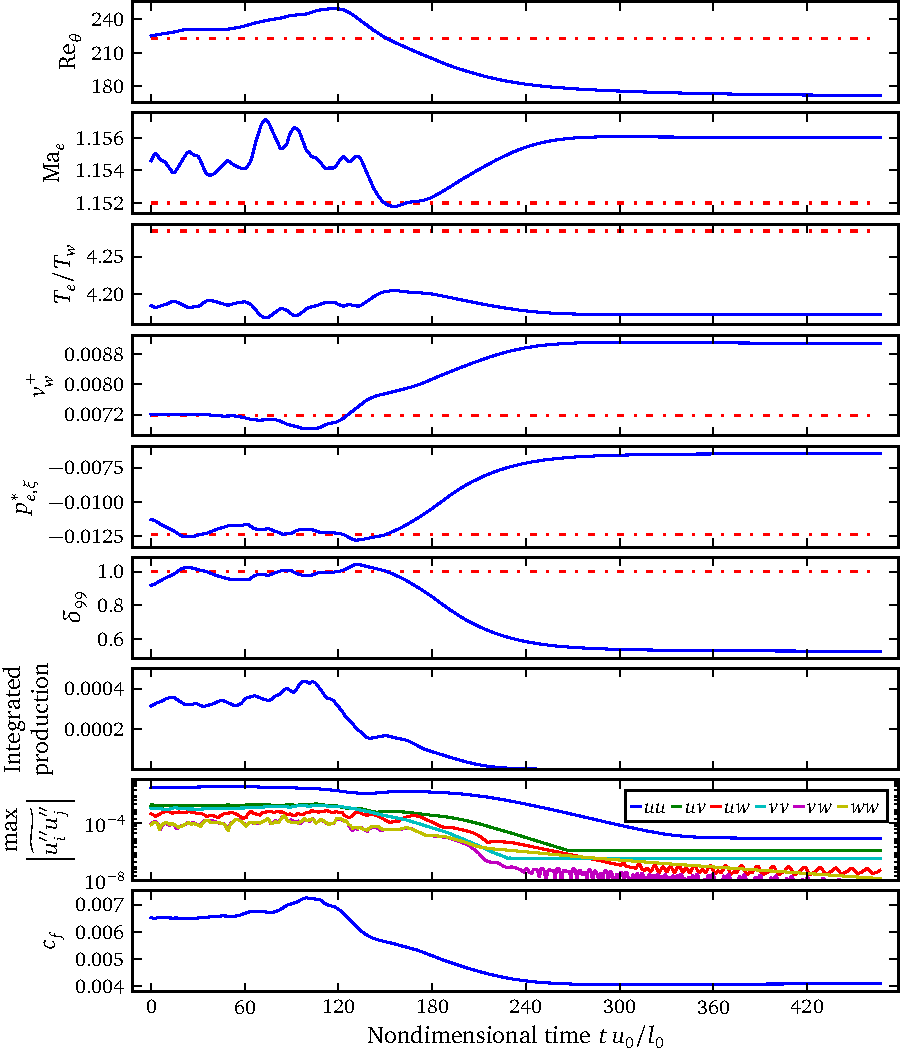
\includegraphics[width=\textwidth]{relam4134}
\caption[Refinement of coarse exploratory simulation for location 4.134~m]{%
    Refinement of exploratory simulation at location 4.134~m.\label{fig:relam4134}
    Dashes mark target conditions.
}
\end{figure}

\begin{figure}
\centering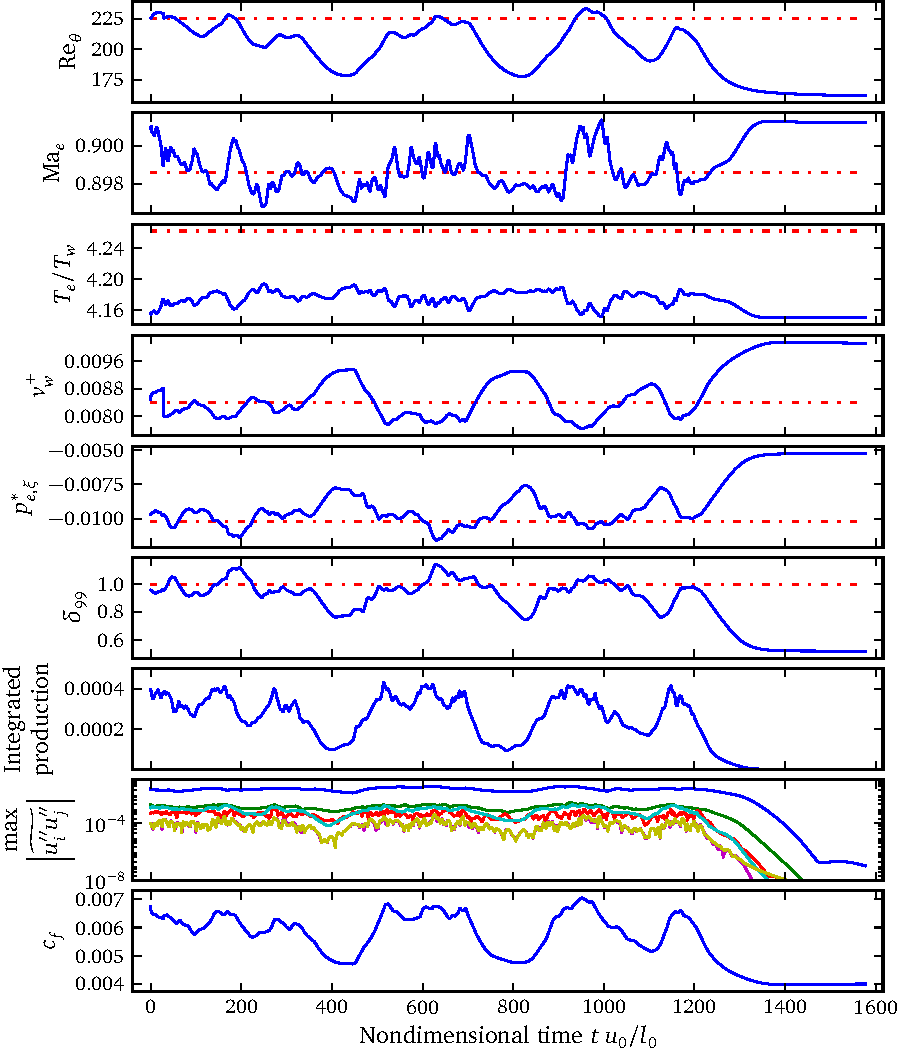
\includegraphics[width=\textwidth]{relam3199}
\caption{Refinement of exploratory simulation for location 3.199~m.\label{fig:relam3199}}
\end{figure}

\begin{figure}
\centering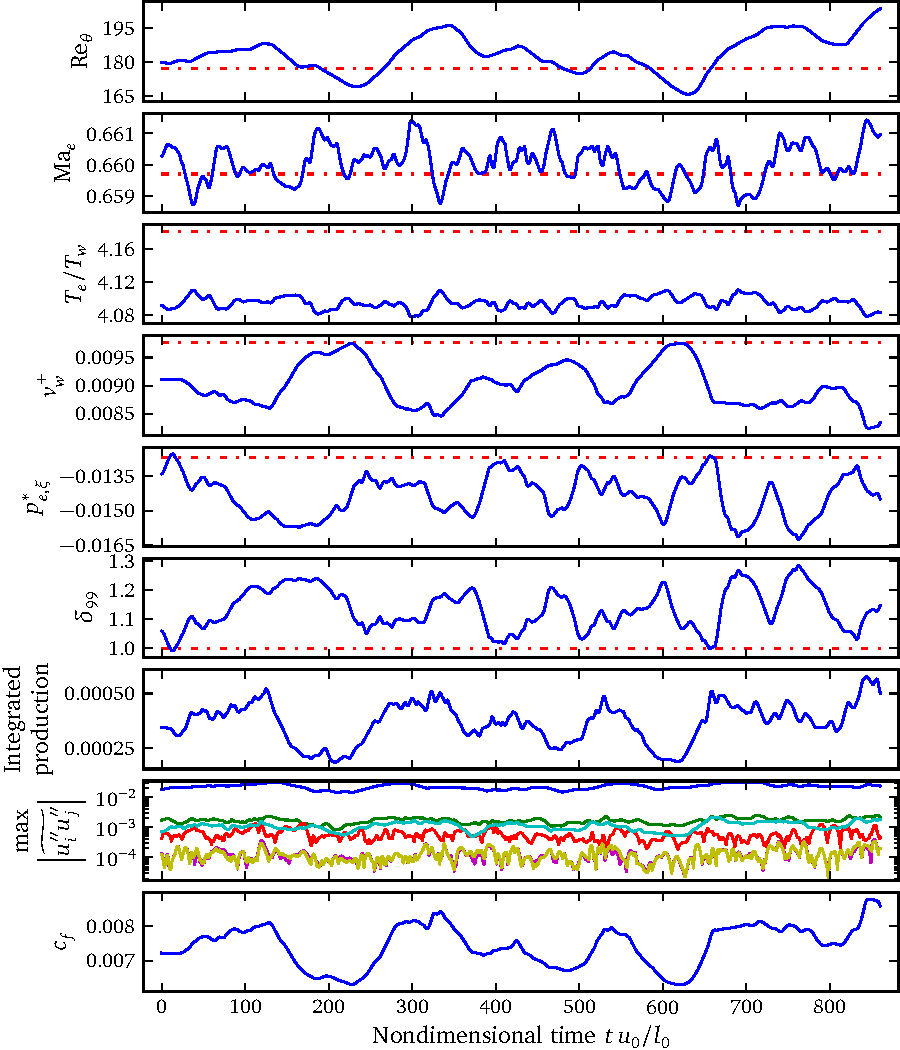
\includegraphics[width=\textwidth]{relam2299}
\caption{Refinement of exploratory simulation for location 2.299~m.\label{fig:relam2299}}
\end{figure}

\begin{figure}
\centering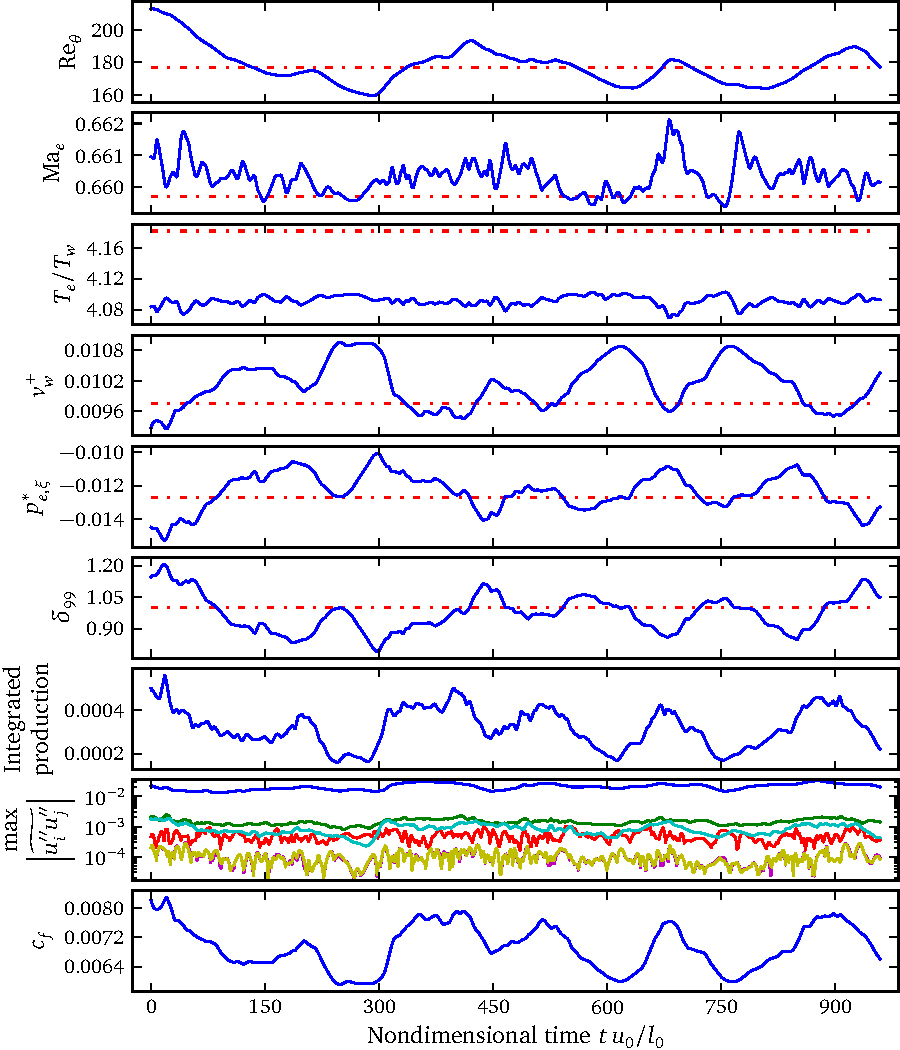
\includegraphics[width=\textwidth]{redux2299}
\caption[Continuation of refinement study for location 2.299~m.]
        {Continuation of refinement study for location 2.299~m.
         Input parameters adjusted to $\Reynolds=1150$,
         $\operatorname{gr}_{t_0}\!\left(\Delta\right)=0.01125$,
         and $v_w/v_0=\num{2.915e-4}$ to better achieve target
         conditions.\label{fig:redux2299}}
\end{figure}


\begin{figure}
\centering
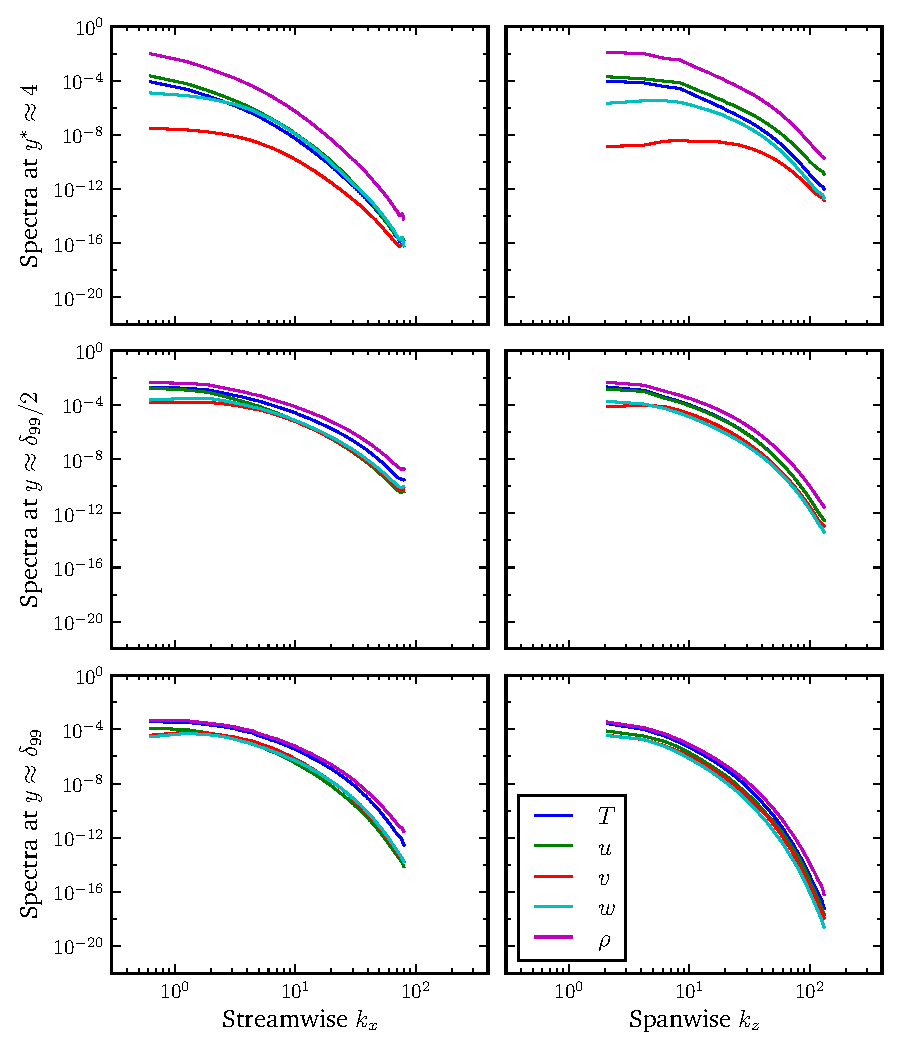
\includegraphics[width=\textwidth]{spectra-redux2299}
\caption{%
    One-dimensional, unnormalized Fourier energy spectra from an ensemble
    over the location 2.299~m data appearing in
    \autoref{fig:redux2299}.\label{fig:spectra-redux2299}
}
\end{figure}

\begin{figure}
\centering
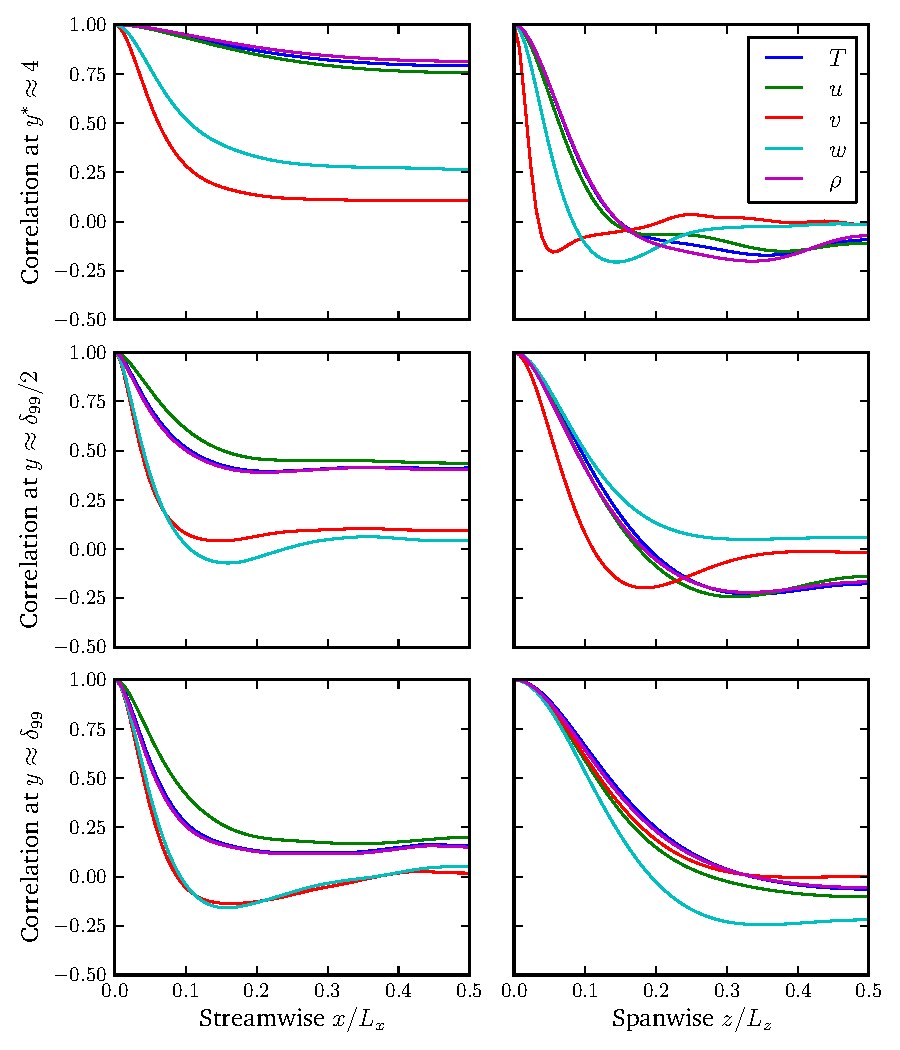
\includegraphics[width=\textwidth]{autocorr-redux2299}
\caption{%
    Two-point correlations from an ensemble over the location 2.299~m data
    appearing in \autoref{fig:redux2299}.\label{fig:autocorr-redux2299}
}
\end{figure}

\begin{figure}
\centering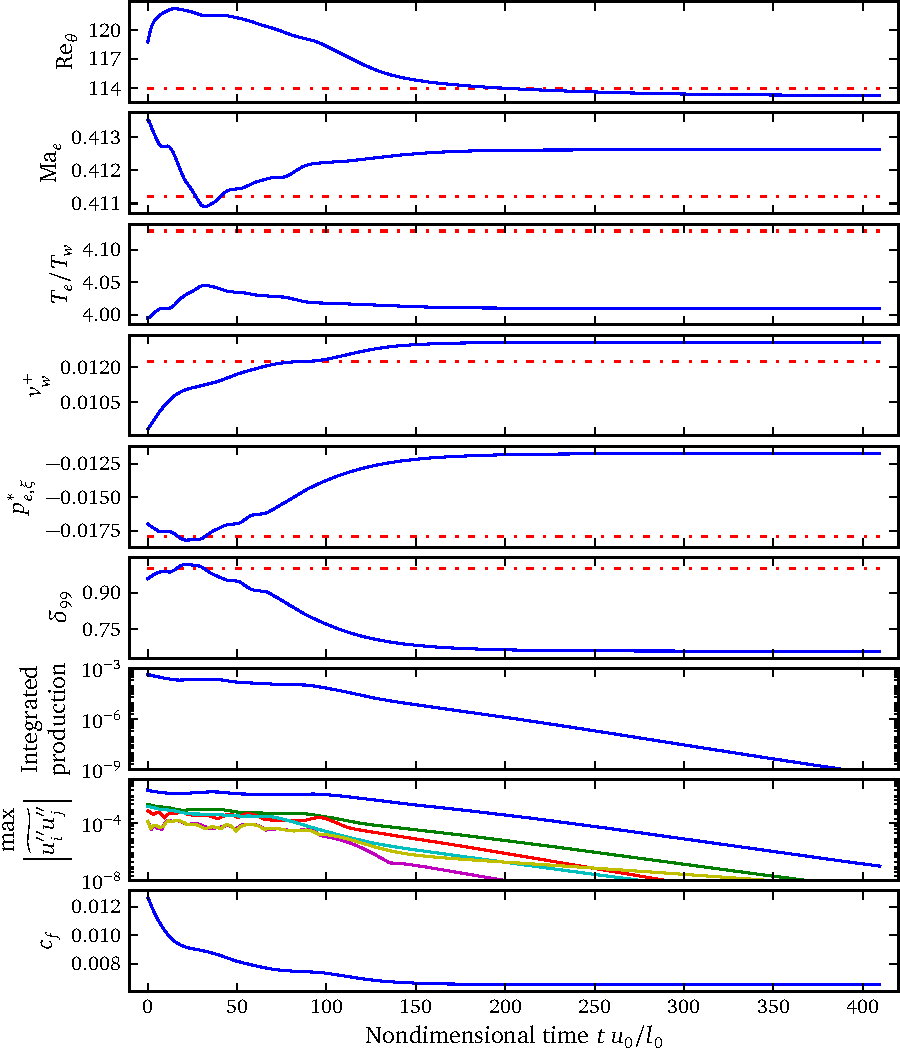
\includegraphics[width=\textwidth]{relam1389}
\caption{Refinement of exploratory simulation for location 1.389~m.\label{fig:relam1389}}
\end{figure}


%%%%%%%%%%%%%%%%%%%%%%%%%%%%%%%%%%%%%%%%%%%%%%%%%%%%%%%%%%%%%%%%%%%%%%%%%%%%%%
\clearpage
\subsection{Results from Fully Turbulent Initial Conditions}
\label{sec:relam_results_turb}

Not one of the post-refinement cases from the prior section used an
initial field known to demonstrate salient turbulent boundary layer
features.  They are, nonetheless, informative.  In particular,
Figures~\ref{fig:relam4134} and~\ref{fig:relam3199} suggest that conditions
4.134~m and 3.199~m both will relaminarize starting from a proper initial field.

Figures~\ref{fig:redux4134} and~\ref{fig:redux3199} on
pages~\pageref{fig:redux4134} and~\pageref{fig:redux3199} investigate those
two locations using stationary turbulent fields from simulations t4.134 and
t3.199, documented in \autoref{sec:bldata}, as initial conditions.
%
Local conditions from \autoref{tbl:cevisslam_inputs} were achieved by setting
the necessary code inputs for initial fully turbulent fields with resolution
$512\times{}256\times{}256$.
%
Because the initial grids, designed for $\Reynolds[\theta]{}=380$ and
531 flows, are excessive for $\Reynolds[\theta]{}\approx225$ they were
coarsened as the simulations proceeded.
%
The 4.134~m case resolution was gradually brought down past
$384\times{}256\times{}192$, past $384\times{}192\times{}192$, and
finally to $256\times{}192\times{}128$ at $t\approx{}34$ where
$\Delta{}x^{+}\approx{}17.2$ and $\Delta{}z^{+}\approx{}10.3$.
%
This case relaminarized after 10.4 turnovers in contrast to 6 observed in
\autoref{fig:relam4134}.
%
The 3.199~m case was handled similarly but was reduced only as
far as $384\times{}192\times{}192$ at $t\approx{}20$ where
$\Delta{}x^{+}\approx{}13.2$ and $\Delta{}z^{+}\approx{}7.9$.
%
This case relaminarized after 13.2 turnovers in contrast to the 36.3 observed in
\autoref{fig:relam3199}.
%
Both simulations used resolutions similar to those in
\autoref{tbl:table_turb_hbl}, which were found adequate.
%
Qualitatively both cases show the same features as the earlier refinement study
did at these locations.  Namely, the supersonic case at 4.134~m smoothly
dissipated away while the subsonic case at 3.199~m had a longer dwell time
before a relatively quick collapse.

For the studied parametrization of Bauman's fully laminar Orion MPCV solution,
locations 4.134~m and 3.199~m represent the boundary layer conditions on the
thermal protection system \emph{a priori} expected most likely to sustain
turbulence.  They possess $\Reynolds[\theta]{}$ within 4.6\% of peak 236 (found
at 3.762~m), among the highest $\Mach$, $T_e/T_w$ within 0.8\% of peak 4.321
(found at 3.983~m), and among the lowest $v_w^{+}$.
%
Given that expectation, having observed 4.134~m and 3.199~m relaminarize from
fully turbulent initial conditions, and having discovered a field
able to sustain nontrivial fluctuations at 2.299~m, the study was halted.

Despite comments made at the end of \autoref{sec:relam_methods}, a subsequent
confirmation of the relaminarizations seen in Figures~\ref{fig:redux4134}
and~\ref{fig:redux3199} at higher resolutions and for larger box sizes was
not performed.  Those comments pertained to the need to assess the sensitivity
of the hypothetical edge of the turbulence sustaining region to changes in
discretization.  Having observed no such edge, that particular sensitivity
became irrelevant.

%Two other sensitivities instead became of interest.
%%
%The first sensitivity question, and the more important one to address, is if
%modifying the domain size changes whether or not some
%given local conditions can sustain turbulence.
%%
%Only examining the impact of choosing a larger domain is of physical interest
%because employing a smaller domain is well-known to encourage aphysical
%simulation artifacts to appear.\footnote{%
%    As is true of many DNS studies, the present work
%    already examined nearly the smallest suitable periodic box.
%}
%%
%Intuitively, a larger domain better approximates the ability of a turbulent spot
%or some other turbulence-inducing disturbance to ``exit'' the simulation by decreasing
%the fraction of the overall periodic domain with which that spot interacts.
%Accordingly, we believe enlarging the domain necessarily increases the tendency
%to relaminarize.
%%
%The second sensitivity question is whether enlarging the domain impacts the time
%to relaminarize.  We suspect, per the same intuition, that larger domains take
%less time to relaminarize.  However, the matter was not pursued as it
%does not impact the following discussion.

\begin{figure}
\centering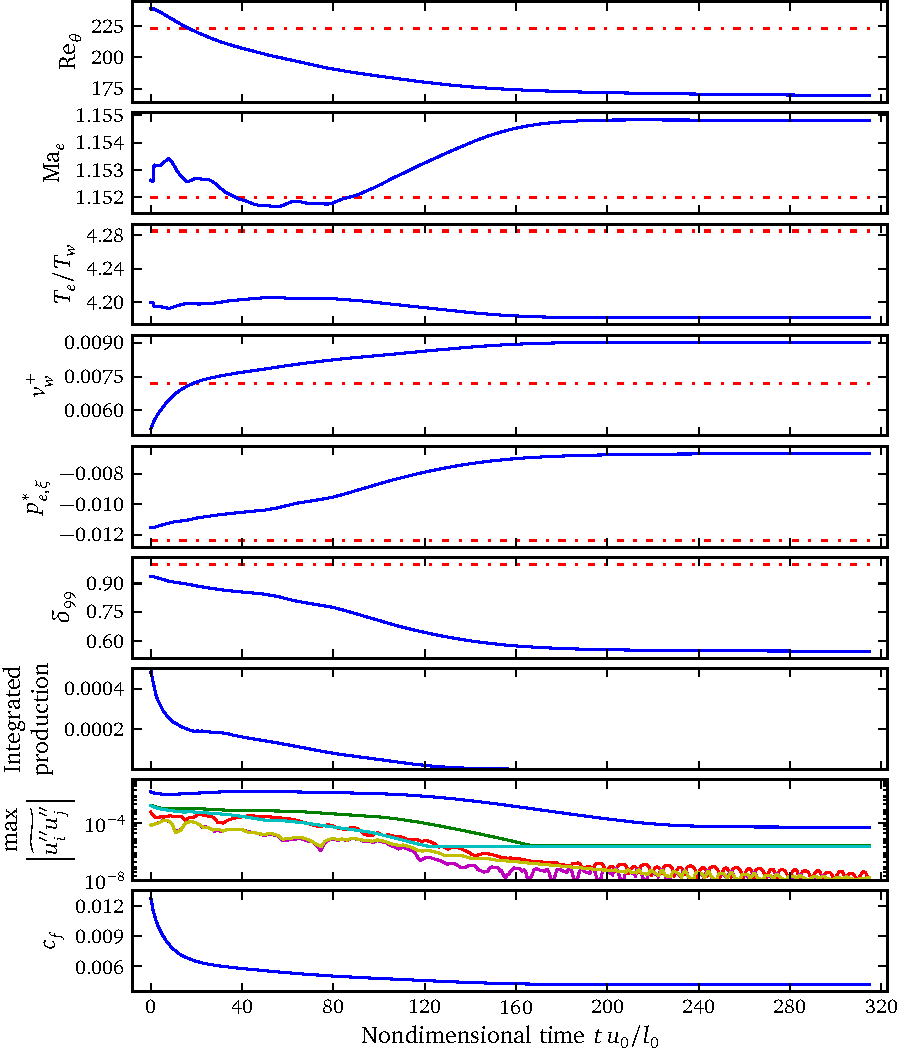
\includegraphics[width=\textwidth]{redux4134}
\caption{Fully turbulent initial condition study for location 4.314~m.\label{fig:redux4134}}
\end{figure}

\begin{figure}
\centering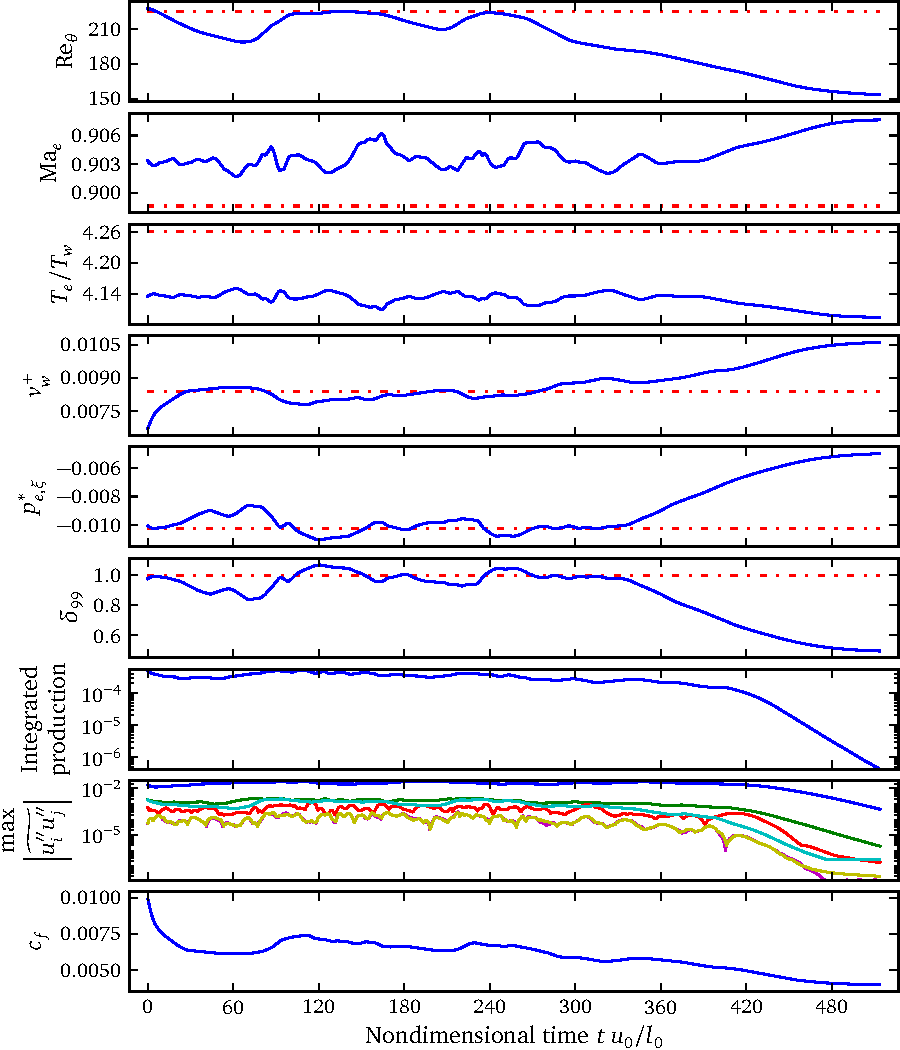
\includegraphics[width=\textwidth]{redux3199}
\caption{Fully turbulent initial condition study for location 3.199~m.\label{fig:redux3199}}
\end{figure}

%%%%%%%%%%%%%%%%%%%%%%%%%%%%%%%%%%%%%%%%%%%%%%%%%%%%%%%%%%%%%%%%%%%%%%%%%%%%%%
\clearpage
\section{Discussion}
\label{sec:relam_discussion}

Given the Orion MPCV boundary layer characterization in
Figures~\ref{fig:cevisslam_summary1} and~\ref{fig:cevisslam_summary_fpg}, that
local conditions at 4.134~m and 3.199~m relaminarized from fully turbulent
initial conditions, as shown in Figures~\ref{fig:redux4134}
and~\ref{fig:redux3199}, suggests no turbulence sustaining region exists on this
particular thermal protection system surface in this particular reentry scenario
according to the present modeling applied per the chosen methodology.  Those two
locations possess among the highest $\Reynolds[\theta]$ found in the Orion MPCV
International Space Station return scenario combined with weak $v_w^{+}$ and
$p_{e,\xi}^\ast$ and were \emph{a priori} anticipated to sustain turbulence if
any portion of the boundary layer could.

How robust is accepting the possible conclusion that the Orion
MPCV is fully laminar in this scenario with respect to using that information to predict aerothermodynamic
heating?  By using turbulent initial conditions in a periodic domain as a
surrogate for a fluctuation-rich flight environment, our methodology attempted
to capture that the reentry vehicle is awash in perturbations from the
freestream, from aerothermochemistry, from ablator outgassing, and from surface
roughness.  Setting aside concerns regarding the verisimilitude of the
homogenized governing equations, the robustness of a fully laminar conclusion
depends to a large extent on whether or not the turbulent initial condition
surrogate was adequate.

Drawing on the nonlinear stability theory discussed in
\autoref{sec:energyperturbationtheory}, turbulent initial conditions were
adopted for the relaminarization study because they are physically relevant but
moreso because they represent large, potentially self-sustaining disturbances
relative to laminar flows.
%
The discovery of the field able to sustain nontrivial
fluctuations at 2.299~m, pictured in \autoref{fig:redux2299}, demonstrates that
turbulent initial conditions were not the most conservative possible way to
emulate a fluctuation-rich flight environment for the purposes of determining
where local conditions can sustain turbulence.  Heightened conservatism is appropriate
because in-flight perturbations cannot be characterized well-enough to apply
transition models as discussed in \autoref{sec:transition}.
%Therefore, though the 2.299~m field was clearly not physical, we believe
%its discovery is germane

Consequently, despite relaminarization from turbulent initial
conditions at 4.134~m and 3.199~m, the existence of a long-lived,
fluctuating field at 2.299~m forces us to conservatively conclude that
the turbulence-sustaining region on the Orion MPCV extends from the
edge of the thermal protection system to at least 2.299~m leeward of
the stagnation point.  Having observed location 1.389~m relaminarize
from initial conditions like those that generated the fluctuation-sustaining
2.299~m field,
we conclude that the turbulence
sustaining region does not extend to within 1.389~m leeward of the
stagnation point.  That conclusion is predicated on the
homogenized governing equations providing accurate predictions regarding
the turbulence-sustaining behavior of spatially evolving boundary layers
which has not been validated in the present work.

Where between locations 1.389~m and 2.299~m is the edge of the turbulence
sustaining region?  We suspect it lies closer to 2.299~m but we do not know
conclusively.
%
Investigating that interval will require a more sophisticated way than
crude auxiliary simulations to determine the code inputs necessary to
incrementally bring the
fluctuation-sustaining 2.299~m field inward towards the stagnation point.
%
Two suggestions were already made in \autoref{sec:relam_methods}.
%
%Indeed, though not shown in the results section, it took three separate attempts
%from \autoref{fig:relam2299} to better achieve its target conditions in
%\autoref{fig:redux2299}.
%
Calibrating a turbulence model equipped with spatiotemporal homogenization terms
to reproduce statistics from the fluctuation-sustaining 2.299~m field appears to be a
necessary first step towards either suggestion.

One factor contributing to the difficulty of obtaining code parameters to
match such local conditions was the implicit dependence of $v_w^{+}$ on
all code inputs.  The present study targeted a constant $v_w^{+}$ based
on conditions found in Bauman's fully laminar Orion MPCV simulation.
The metric was selected because it approximated outgassing from a
steady ablative heat shield.  As can be seen from the results,
the normalized wall blowing became stronger as simulations relaminarized.
A better approach for future work may be to control $v_w/u_0$ to match the
local nondimensional heat flux $B_q$~\citep{Bradshaw1977Compressible}
from MPCV data.
Matching the heat flux approximates an ablator able to react to flow
conditions.  Care is required, however, to not have the controller
mechanism introduce undesirable time scales into the simulation.
%\footnote{%
%    The idea of using a controller to hold $\delta_{99}/l_0\approx{}1$
%    was entertained long enough to prepare an implementation
%    (\url{https://github.com/RhysU/helm}) along with much of the
%    required infrastructure within Suzerain.  The idea was abandoned
%    after coming to believe turning the controller for this study
%    would require time commensurate with simply adjusting the
%    $\operatorname{gr}_{t_0}\left(\Delta\right)$ and, done hurriedly,
%    could destabilize the simulations.
%}

It would be interesting to repeat the \citet{Bauman2011Loose} heat shield
simulations with turbulence tripped at 1.389~m and to compare the result with
both \autoref{fig:normalized_difference} and \autoref{tbl:BaumanCEVConditions}.
That prediction could be contrasted with heating data gathered during the
upcoming NASA Exploration Flight Test-1~\citep{SpaceCom20140317} in the hope
that the simulation matches evidence of where on the heat shield
turbulence-enhanced energy transport is present.
%
However, a comparison may not be straightforward as that flight test will use a
different reentry trajectory than the peak heating regime studied here.

Finally, if one wanted to limit a relaminarization study to only fully turbulent
initial conditions and possibly find a turbulence-sustaining edge, the higher
speed Exploration Flight Test-1 trajectory may be ideal.  Studying a faster
trajectory with the suggested methodology improvements may allow interrogating
the physics at the cusp where turbulence can only barely be sustained.
